\begin{figure}
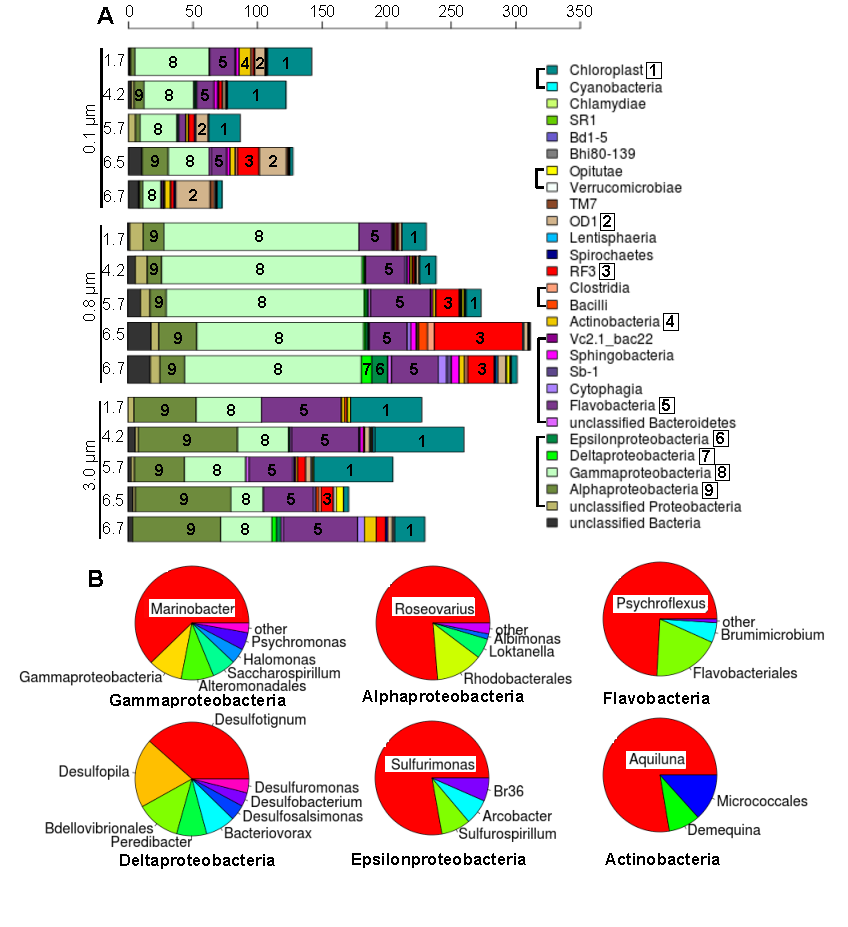
\includegraphics[width=\textwidth]{orglake_figures/genus_barplots3_1.pdf}
\caption[Diversity of \emph{Bacteria} and \emph{Eucarya} in Organic Lake]{Diversity of (\textbf{A}) \emph{Bacteria} and (\textbf{B}) \emph{Eucarya} from each size fraction (0.1, 0.8 and 3.0 \textmu{}m) at each sample depth (1.7, 4.2, 5.7, 6.5 and 6.7 m) of Organic Lake aggregated according to class. The x-axis shows counts of \ac{SSU} normalised to average reads acquired per sample filter. Taxa that belong to the same higher rank are shown grouped with a square bracket in the legend. Abundant taxa are labelled in plot with a number that corresponds to the numbered boxes in the legend. (\textbf{C}) Composition of abundant bacterial classes.}
\label{fig:genus_barplots}

\end{figure}
